\chapter{Introduzione alla Programmazione Concorrente}

\section{Il corso in breve...}

\subsection{Cosa si intende per programmazione concorrente?}

La programmazione concorrente nasce con i \fancyglitter{sistemi concorrenti} nell'ambito dei \newfancyglitter{sistemi operativi} con il concetto di \newfancyglitter{processo} (o \newfancyglitter{thread}). 

\dfn{Sistema concorrente}{
  Un sistema concorrente è un sistema \newfancyglitter{software} implementato su una \newfancyglitter{piattaforma hardware} in grado di eseguire \textbf{\newfancyglitter{contemporaneamente}} più attività diverse che condividono \newfancyglitter{risorse comuni}\footnote{Porzioni di memoria centrale, CPU, etc.}. 
}

\nt{Un esempio di sistemi concorrenti sono i \newfancyglitter{sistemi operativi multiprogrammati}.}

\cor{Programma concorrente}{Un programma concorrente è un insieme di \evidence{moduli sequenziali} che possono essere eseguiti in parallelo.}

\subsubsection{Tipi di parallelismo:}

\begin{itemize}
  \item [$\Rightarrow$] \newfancyglitter{Parallelismo reale}: l'esecuzione dei moduli è realmente sovrapposta nel tempo;
  \item [$\Rightarrow$] \newfancyglitter{Parallelismo apparente}: si applica la tecnica di \fancyglitter{interleaving delle istruzioni}.
\end{itemize}

\nt{In entrambi i casi il termine \fancyglitter{concorrenza} si utilizza come un'astrazione per studiare il parallelismo.
}

\subsubsection{In questo corso si tratterà di:}

\begin{itemize}
  \item Introduzione ai \fancyglitter{principi} della programmazione concorrente;
  \item Analisi dei principali \fancyglitter{costrutti linguistici} per la programmazione concorrente;
  \item Applicazione di questi costrutti a vari problemi di \fancyglitter{sincronizzazione} e \fancyglitter{comunicazione} in programmi concorrenti;
  \item Studio delle \fancyglitter{proprietà di correttezza} dei programmi concorrenti: \newfancyglitter{no deadlock}, \newfancyglitter{no starvation}, etc. 
\end{itemize}

\subsection{Cosa si intende per algoritmo distribuito?}

\dfn{Sistema distribuito}{
  Un sistema distribuito è un sistema composto da \newfancyglitter{più computer} che non condividono la memoria o altre risorse, ma sono connessi da canali di comunicazione\footnote{Debolmente connessi.}.
}

\cor{Algoritmo distribuito}{
  Un algoritmo distribuito è un algoritmo progettato per essere eseguito da un sistema distribuito.
}

\begin{figure}[h]
    \centering
    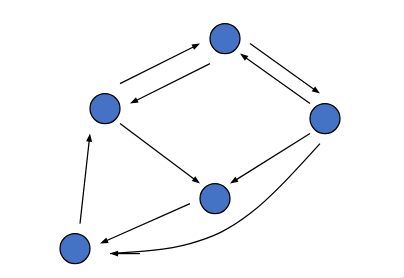
\includegraphics[scale=0.4]{01-IntroduzioneAllaProgrammazioneConcorrente/AlDist.png}
    \caption{Schema di un sistema distribuito}
\end{figure}

\subsubsection{Obiettivi per la parte di corso di algoritmi distribuiti:}

\begin{itemize}
\item Introduzione di modelli formali che permettano l'analisi di \fancyglitter{algoritmi distribuiti di base};
\item Studio della \fancyglitter{correttezza} e delle \fancyglitter{prestazioni} degli algoritmi distribuiti presentati;
\item Analisi di \fancyglitter{algoritmi distribuiti} in presenza di \fancyglitter{malfunzionamenti} (algoritmi fault tolerant).
\end{itemize}

\section{Parallelismo}

\subsection{Interleaving di Istruzioni Atomiche}

\dfn{Processo}{
  Modulo \newfancyglitter{sequenziale} di un programma concorrente (a volte si usa il termine thread).
}

\nt{Per gli scopi di questo corso processo e thread vengono assunti come sinonimi.}

\begin{figure}[h]
    \centering
    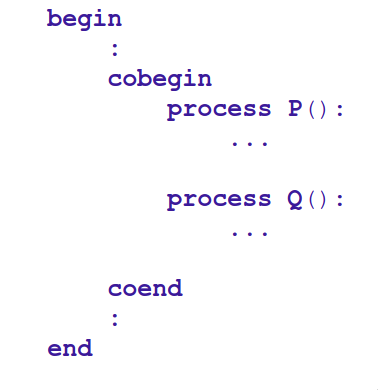
\includegraphics[scale=0.3]{01-IntroduzioneAllaProgrammazioneConcorrente/C1.png}
    \caption{Pseudocodice}
\end{figure}


\begin{figure}[h]
    \centering
    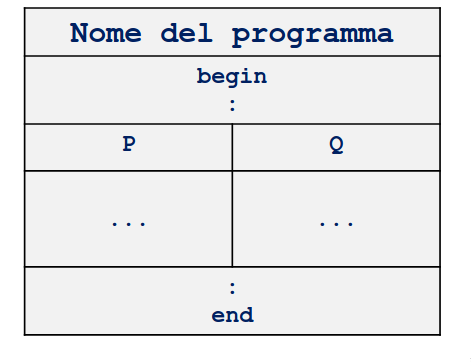
\includegraphics[scale=0.3]{01-IntroduzioneAllaProgrammazioneConcorrente/C2.png}
    \caption{Tabella}
\end{figure}

\qs{}{Che cos'è l'interleaving?}

\dfn{Interleaving}{Si suppone che ogni esecuzione di un programma concorrente sia ottenuta \newfancyglitter{interfogliando in maniera arbitraria} le istruzioni dei vari processi.}

\nt{Il risultato dell'interleaving è detto \fancyglitter{computazione} o \fancyglitter{scenario}.}

\ex{Quante persone sono entrate in laboratorio?}{
Si ha un laboratorio con due tornelli che hanno un contatore condiviso che viene incrementato di 1 quando entra una persona.
  \begin{center}
    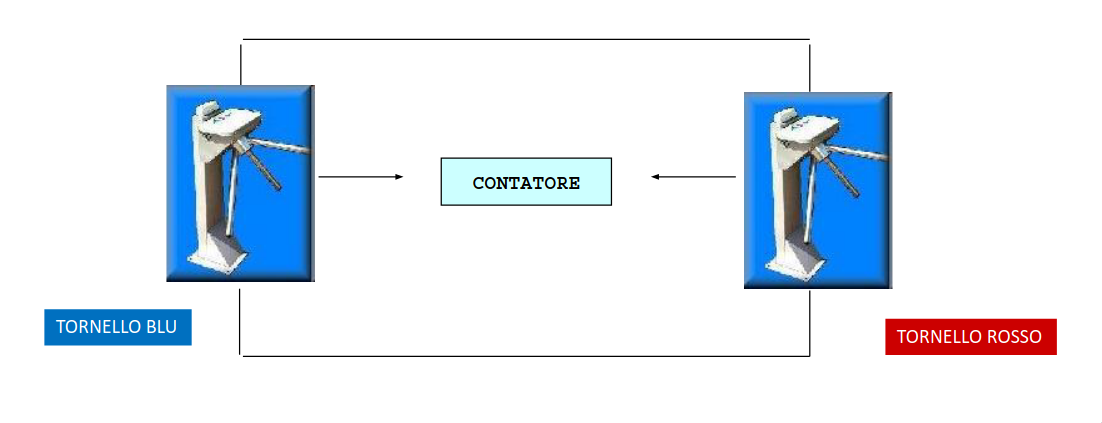
\includegraphics[scale=0.3]{01-IntroduzioneAllaProgrammazioneConcorrente/Lab.png}
\end{center}

Si inizia dichiarando la variabile condivisa \textit{counter} (inizializzata a 0). Dopo di ché si suppone che il tornello blu faccia entrare 100 persone e il tornello rosso altre 100.

\begin{center}
    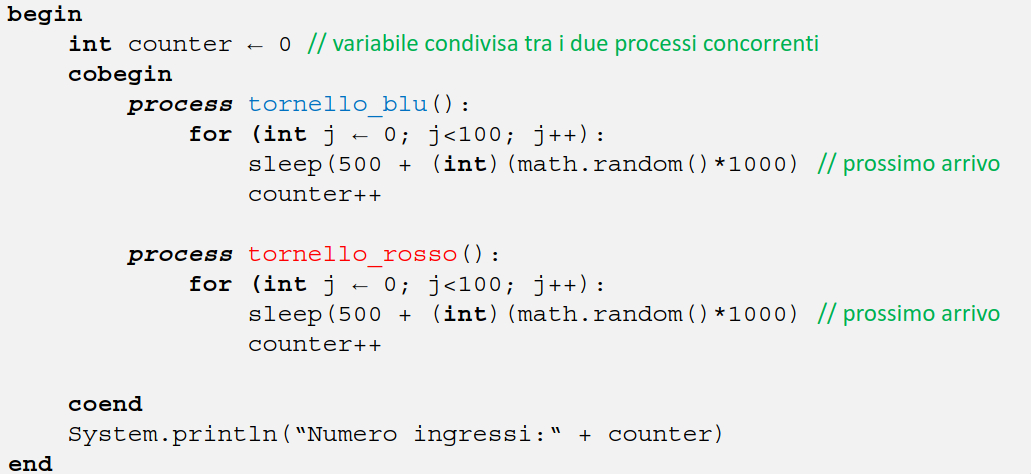
\includegraphics[scale=0.3]{01-IntroduzioneAllaProgrammazioneConcorrente/LabC1.png}
\end{center}

\begin{center}
    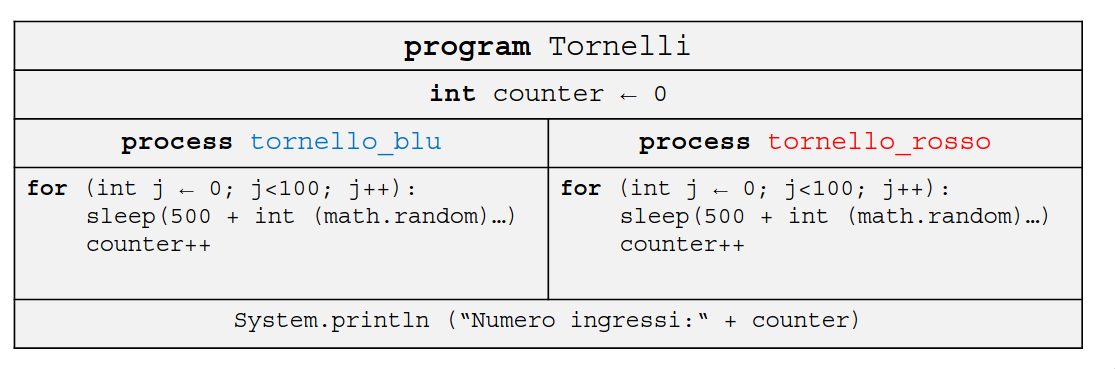
\includegraphics[scale=0.3]{01-IntroduzioneAllaProgrammazioneConcorrente/LabC2.png}
\end{center}

Alla fine della simulazione verrà stampato il valore 200? Dipende. 

\begin{itemize}
  \item Se l'istruzione \textbf{counter++} è atomica e indivisibile verrà stampato il valore 200;
  \item Ma se fosse realizzata mediante più load, add e store? In tal caso non è garantito che il risultato sarà 200.
\end{itemize}

}

\dfn{Istruzione atomica}{
  Un'istruzione viene detta atomica se viene sempre eseguita interamente senza possibilità di interruzioni\footnote{No interleaving.}.
}

\nt{Il risultato dell'esecuzione "simultanea" di due istruzioni atomiche è lo stesso che si otterrebbe dalla loro esecuzione sequenziale indipendentemente dall'ordine. In generale si assumerà che gli assegnamenti e le valutazioni di espressioni logiche siano operazioni atomiche.} 

\ex{Possibile computazione}{

\begin{center}
    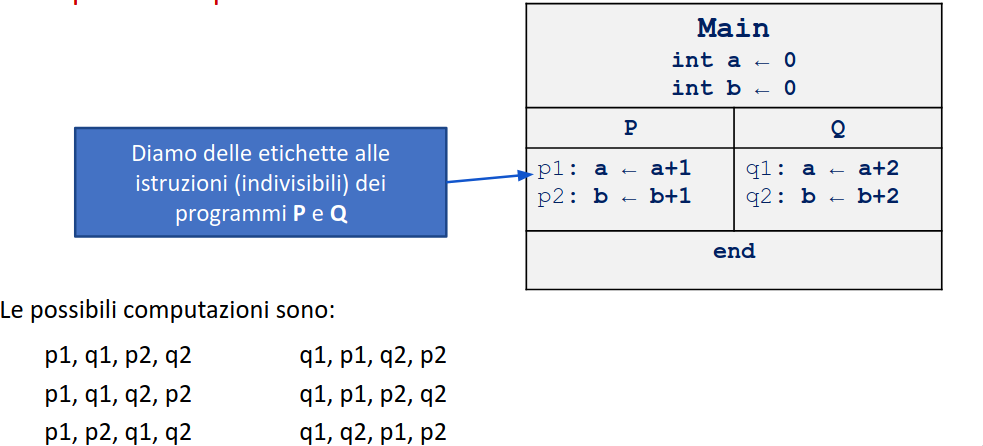
\includegraphics[scale=0.4]{01-IntroduzioneAllaProgrammazioneConcorrente/Comp.png}
\end{center}
È importante notare che p2 non può precedere p1 e q2 non può precedere q1.

\begin{center}
    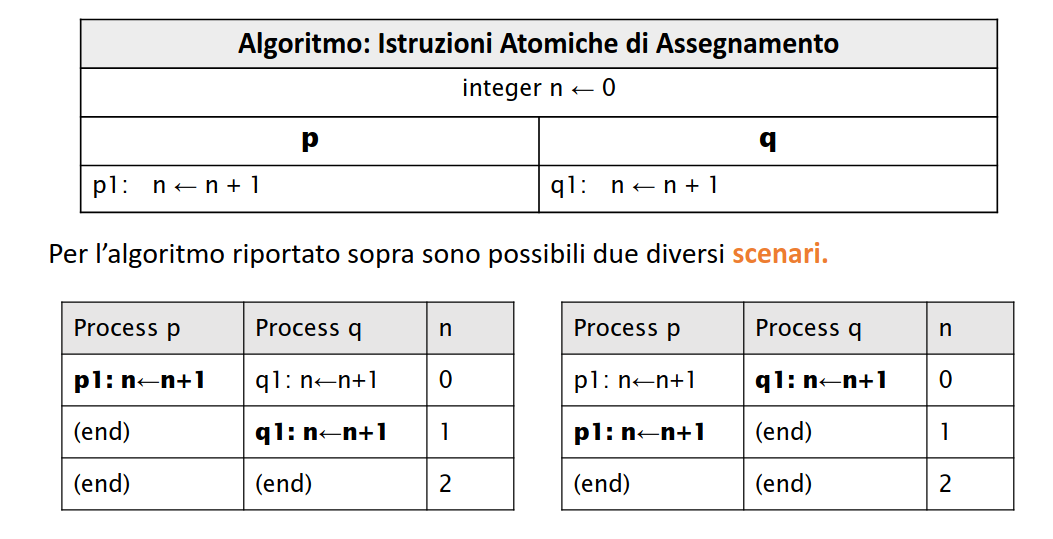
\includegraphics[scale=0.4]{01-IntroduzioneAllaProgrammazioneConcorrente/Comp2.png}
\end{center}

In entrambi i casi sia avrà sempre n = 2 come valore finale. 


\begin{center}
    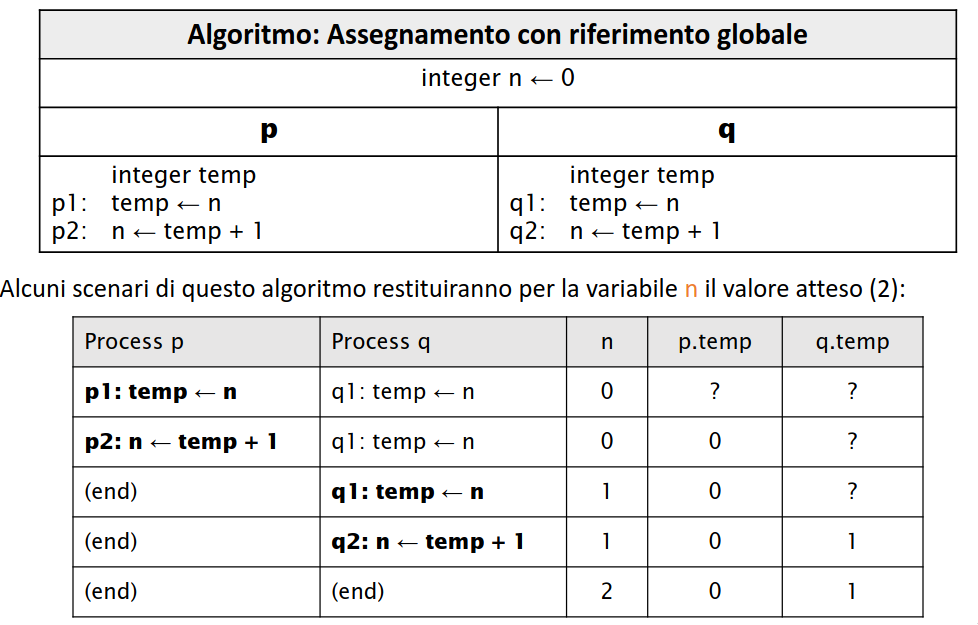
\includegraphics[scale=0.4]{01-IntroduzioneAllaProgrammazioneConcorrente/Comp3.png}
\end{center}

\begin{center}
    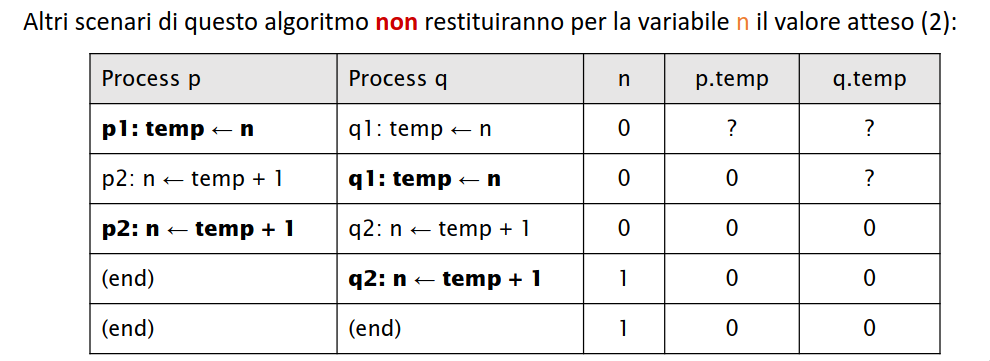
\includegraphics[scale=0.4]{01-IntroduzioneAllaProgrammazioneConcorrente/Comp4.png}
\end{center}

In questo secondo algoritmo l'ordine di esecuzione influenza il risultato. Per cui avere operazioni atomiche non è sufficente a garantire consistenza a un programma concorrente.

}

\nt{Il comportamento osservato nel secondo algoritmo prende il nome di \fancyglitter{race condition} (condizione di corsa).}

\subsection{Sistemi Monoprocessore e Sistemi Multiprocessore}

\subsubsection{Sistemi monoprocessore (parallelismo apparente):}

\begin{itemize}
  \item i processi sono \fancyglitter{alternati nel tempo} per \newfancyglitter{simulare} un multiprocessore;
  \item in ogni istante un solo processo è in esecuzione;
  \item c'è interleaving nell'esecuzione delle singole istruzioni;
  \item il meccanismo degli \fancyglitter{interrupt} su cui è basato l'avvicendamento dei processi garantisce che l'interrupt venga servito primo o dopo l'esecuzione di un'istruzione, mai durante;
  \item ogni istruzione macchina è \fancyglitter{atomica}.
\end{itemize}

\subsubsection{Sistemi multiprocessore con memoria comune (parallelismo reale):}

\begin{itemize}
  \item più processi vengono eseguiti \fancyglitter{simultaneamente} su processori diversi;
  \item c'è \fancyglitter{sovrapposizione} (overlapping) nell'esecuzione delle istruzioni;
  \item i processi sono \fancyglitter{sequenzializzati nell'accesso alla memoria};
  \item le operazioni elementari (\textit{microistruzioni}) che implementano istruzioni macchina sono realizzate da CPU diverse, ma le operazioni elementari che consistono in accessi alla memoria devono essere eseguite una alla volta;
  \item in questo caso è l'\fancyglitter{arbitro del bus} che si preoccupa della sequenzializzazione e che garantisce l'atomicità delle operazioni di lettura/scrittura;
  \item l'accesso fisico al bus può rendere atomiche le istruzioni macchina.
\end{itemize}

\nt{In entrambi i sistemi non è possibile prevedere l'alternanza nell'esecuzione di due processi.}

\ex{Programma concorrente}{

\begin{center}
    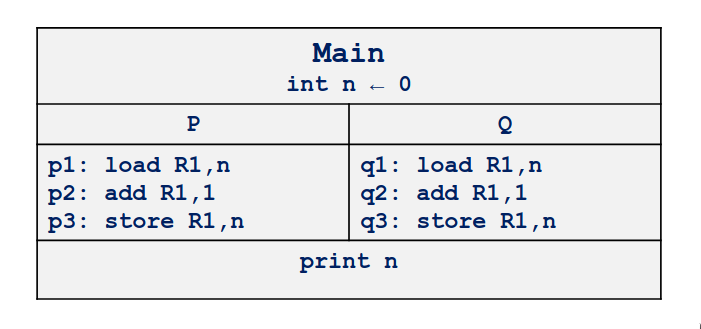
\includegraphics[scale=0.5]{01-IntroduzioneAllaProgrammazioneConcorrente/PC1.png}
\end{center}

\begin{center}
    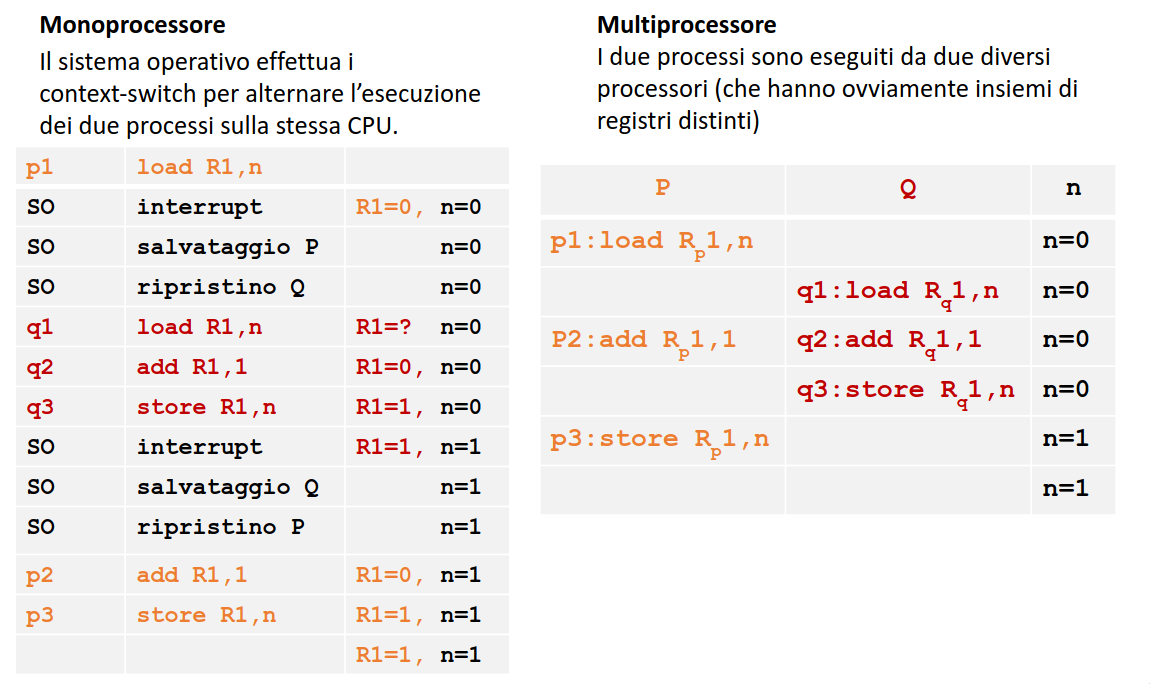
\includegraphics[scale=0.4]{01-IntroduzioneAllaProgrammazioneConcorrente/PC2.png}
\end{center}


}

\qs{}{Le istruzioni macchina sono atomiche?}

\ex{exc}{

\begin{center}
    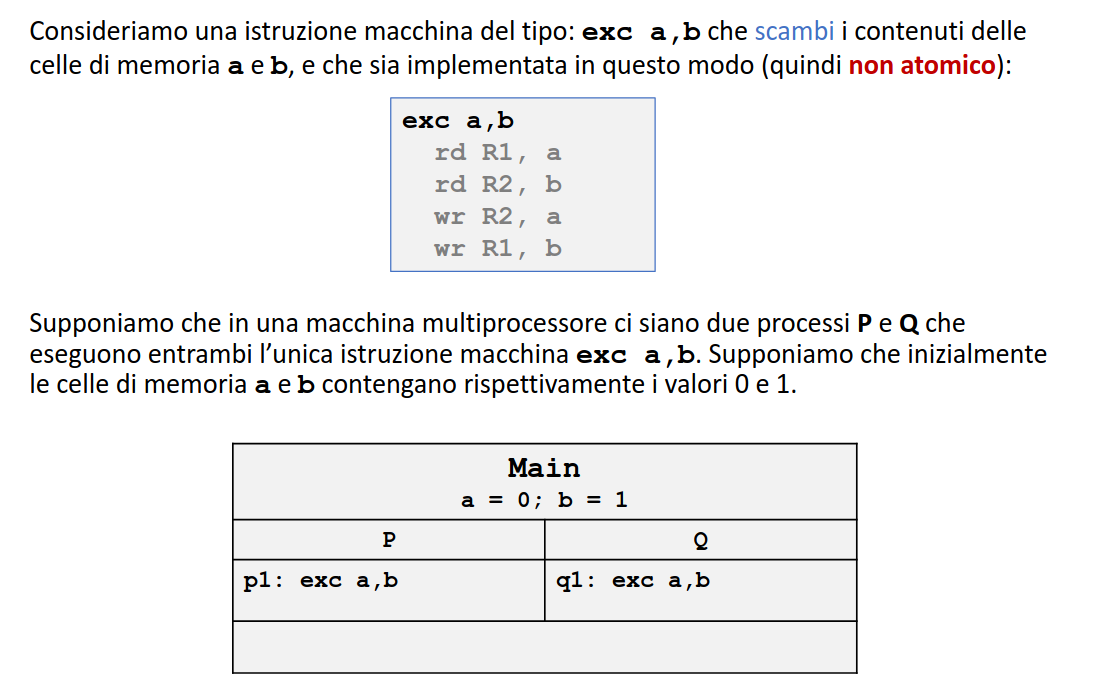
\includegraphics[scale=0.4]{01-IntroduzioneAllaProgrammazioneConcorrente/PE1.png}
\end{center}

\begin{center}
    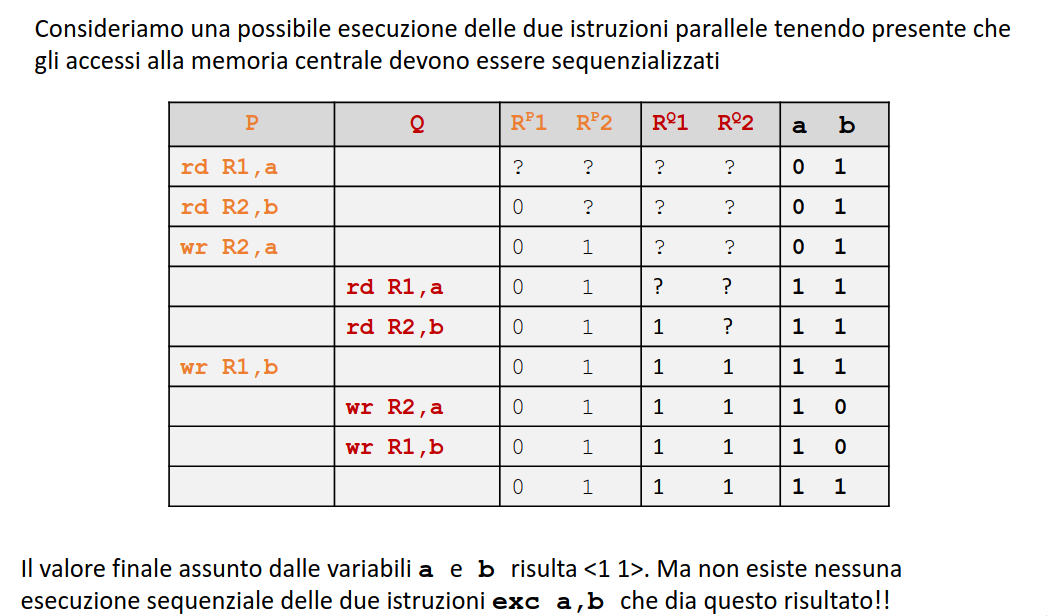
\includegraphics[scale=0.4]{01-IntroduzioneAllaProgrammazioneConcorrente/PE2.png}
\end{center}


}

\dfn{Stato di un programma concorrente}{
  Lo stato di un programma concorrente è una tupla costituita dai valori dei \newfancyglitter{control pointer}\footnote{Indica lo statement del processo che sta per essere eseguito.} dei vari processi e dai valori delle variabili locali e globali.
}

\cor{Transizione}{
  Siano $s_1$ e $s_2$ due stati di un programma concorrente. Esiste una \evidence{transizione} da $s_1$ a $s_2$, indicata con \evidence{$s_1 \to s_2$}, se l'esecuzione di una istruzione nello stato $s_1$ porta nello stato $s_2$.
}

\ex{Programma concorrente banale}{

\begin{center}
    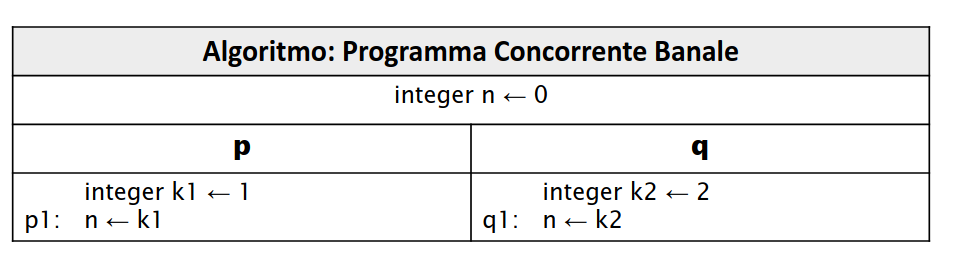
\includegraphics[scale=0.4]{01-IntroduzioneAllaProgrammazioneConcorrente/PCB.png}
\end{center}
\begin{itemize}
  \item Lo stato deve includere i valori dei control pointers (p1 e q1) dei 2 processi, il valore della variabile globale n e i valori delle variabili locali k1 e k2;
  \item Lo stato iniziale può transire da 2 diversi stati a seconda di quale processi esegua per primo l'assegnamento;
  \item Si può illustrare il comportamento di questo programma concorrente con un \fancyglitter{diagramma degli stati}.
\end{itemize}
\begin{center}
    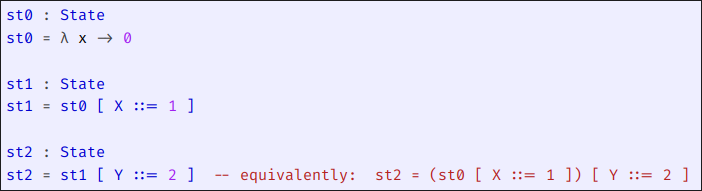
\includegraphics[scale=0.4]{01-IntroduzioneAllaProgrammazioneConcorrente/Stati.png}
\end{center}

}

\section{Correttezza di Programmi Concorrenti}

\subsection{Introduzione e Proprietà}

La definizione di \fancyglitter{correttezza totale} di un programma sequenziale richiede che il programma \fancyglitter{termini} e che, per ogni input, il \fancyglitter{risultato} restituito dal programma sia il valore della funzione che il programma deve calcolare. Purtoppo questa definizione non è adeguata al caso dei programmi concorrenti:

\begin{itemize}
  \item può essere desiderabile che un programma concorrente non termini (ad esempio i processi server degli OS);
  \item inoltre un programma concorrente non può più essere considerato una funzione perché si aggiungono richieste come \fancyglitter{mutua esclusione}, l'assenza di \fancyglitter{deadlock}, l'assenza di \fancyglitter{starvation}.
\end{itemize}

\nt{La correttezza di un programma concorrente viene definita in termini di \fancyglitter{validità di proprietà}.}

\subsubsection{Lampton ha definito due categorie di proprietà di correttezza:}
\begin{itemize}
  \item \fancyglitter{Safety}: la proprietà P deve sempre essere vera (P è vera in ogni stato della computazione);
  \item \fancyglitter{Liveness}: la proprietà P prima o poi sarà vera (in ogni computazione esiste uno stato in cui P è vera).
\end{itemize}

\qs{}{Questo programma termina per tutte le computazioni?}


\begin{center}
    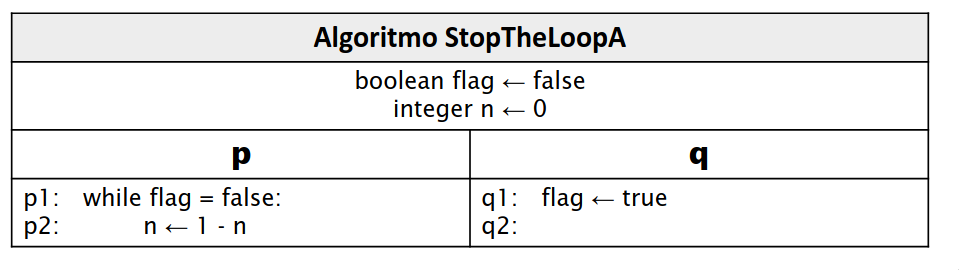
\includegraphics[scale=0.4]{01-IntroduzioneAllaProgrammazioneConcorrente/STL.png}
\end{center}

\nt{Per rispondere dobbiamo vedere il diagramma degli stati corrispondente.}

\begin{center}
    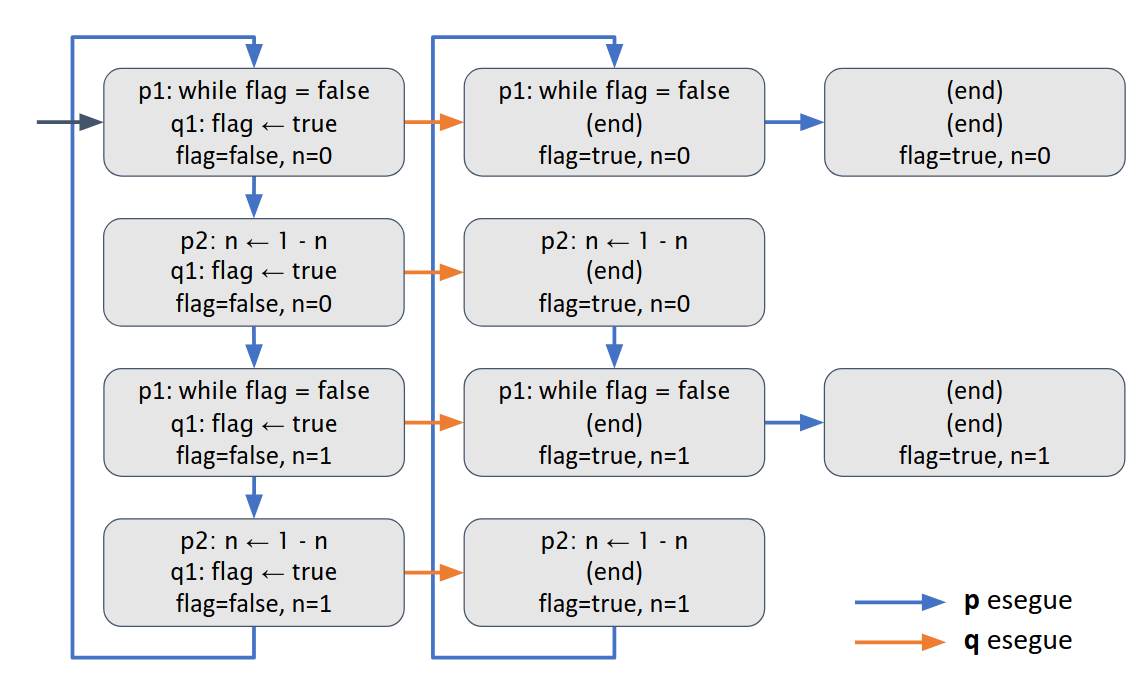
\includegraphics[scale=0.3]{01-IntroduzioneAllaProgrammazioneConcorrente/STL2.png}
\end{center}

\paragraph{Risposta:} questo programma termina solo in due stati, quindi la risposta è no.

\nt{Questo comportamento non è \fancyglitter{fair}.}


\begin{center}
    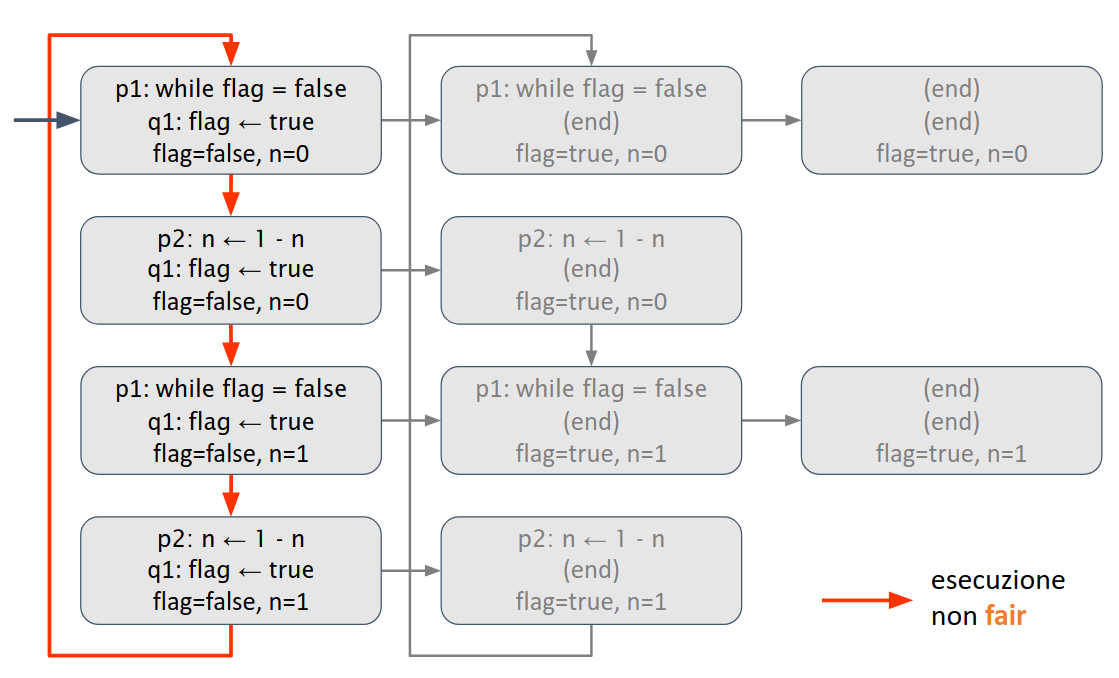
\includegraphics[scale=0.3]{01-IntroduzioneAllaProgrammazioneConcorrente/STL3.png}
\end{center}

\dfn{Fairness}{
  Una computazione è \newfancyglitter{fair} se per ogni istruzione "costantemente" abilitata esiste uno stato in cui essa viene eseguita, prima o poi.
}

\nt{Imporre le \fancyglitter{ipotesi di fairness} a un programma concorrente significa escludere dalle sue computazioni quelle che non soddisfano la proprietà di fairness.}

\subsection{La Correttezza di Programmi}

\subsubsection{La correttezza di un \fancyglitter{programma sequenziale} richiede:}

\begin{enumerate}
  \item Terminazione;
  \item Correttezza del risultato.
\end{enumerate}

\dfn{Program testing}{
  Per controllare la correttezza di un programma sequenziale si può:

  \begin{itemize}
    \item eseguire il programma n volte con dei \newfancyglitter{punti di break} in modo da individuare eventuali malfunzionamenti (debugging) o testare con input predefiniti (unit test);
    \item ricorrere a metodi di verifica (\newfancyglitter{program verification}) basati su sistemi formali, per esempio la logica dei predicati.
  \end{itemize}

}

\nt{La correttezza di un programma concorrente richiede la verifica di opportune proprietà per ogni possibile sua computazione, per cui le tecniche di debugging sono inefficienti.}

\subsubsection{Per provare la correttezza di un programma concorrente si possono usare:}

\begin{itemize}
  \item \fancyglitter{Diagramma degli stati}: però spesso si hanno troppi stati ed è difficile verificare le proprietà di Liveness;
  \item \fancyglitter{Metodi formali di verifica}: prove di proprietà scritte in un adeguato linguaggio logico, basate su invarianti;
  \item \fancyglitter{Model checker}: un programma che costituisce il diagramma degli stati di un programma concorrente e simultaneamente verifica le proprietà. 
\end{itemize}

\subsection{Il Problema della Mutua Esclusione}

\dfn{Problema della mutua esclusione}{
  Se un proceso esegue la propria sezione critica, nessun altro processo esegue la propria.
}

\nt{N processi concorrenti eseguono in un loop infinito una sequenza di statement che può essere divisa in due sotto-sequenze: non-sezione critica (NCS) e sezione critica (CS).}

\begin{center}
    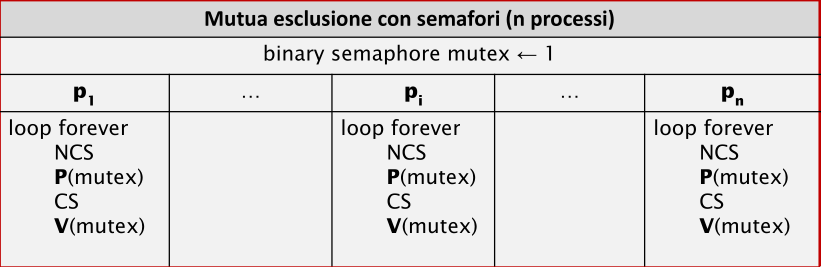
\includegraphics[scale=0.45]{01-IntroduzioneAllaProgrammazioneConcorrente/ME.png}
\end{center}

\dfn{Sincronizzazione}{
  Per ottenere la mutua esclusione si deve introdurre un \newfancyglitter{meccanismo di sincronizzazione}, costituito da statement aggiuntivi, alcuni posti prima dell'accesso alla sezione critica: \newfancyglitter{prologo} (preprotocol) e alcuni all'uscita della sezione critica : \newfancyglitter{epilogo} (postprotocol).
}

\begin{center}
    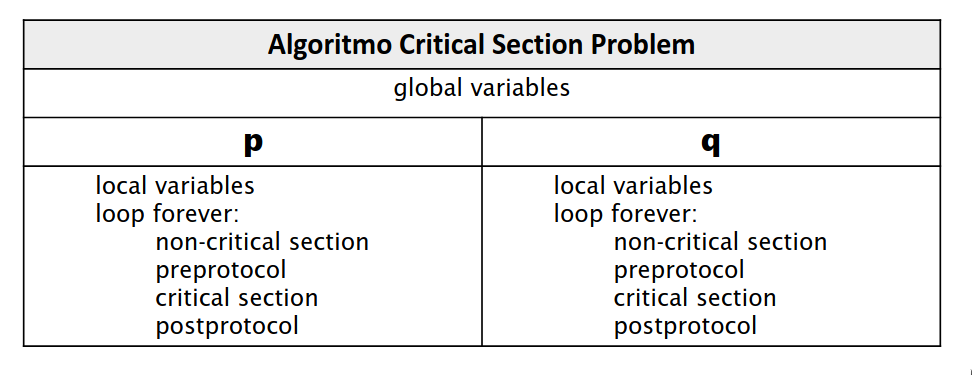
\includegraphics[scale=0.45]{01-IntroduzioneAllaProgrammazioneConcorrente/ME2.png}
\end{center}

\subsubsection{Per risolvere il problema della mutua esclusione si parte da alcune assunzioni:}

\begin{enumerate}
  \item quando un processo è in CS progredisce nell'esecuzione del suo codice e lo porta a termine (non ci sono loop infiniti, statement di terminazione o malfunzionamenti) (\fancyglitter{proprietà di progresso all'interno della sezione critica});
  \item le computazioni sono fair;
  \item le variabili usate nel prologo e nell'epilogo non sono utilizzate in CS o in NCS;
  \item i processi utilizzano sempre correttamente il protocollo.
\end{enumerate}


\begin{center}
    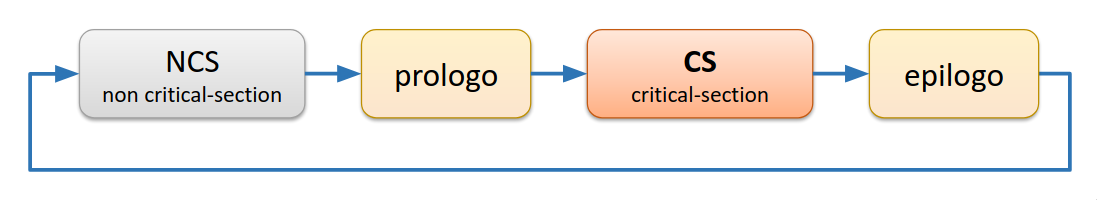
\includegraphics[scale=0.45]{01-IntroduzioneAllaProgrammazioneConcorrente/ME3.png}
\end{center}

\nt{
\begin{itemize}
  \item Se un utente si blocca in CS l'intero sistema si blocca o va in contro a malfunzionamenti;
  \item Le assunzioni 1 e 2 garanticono che nelle CS non si presentino malfunzionamenti, cicli infiniti, statement di terminazione, etc.);
  \item Non si fanno restrizioni sul codice in NCS;
  \item La quarta assunzione garantisce che i protocolli proposti siano sempre eseguiti;
  \item La terza assunzione garantisce che le variabili del protocollo siano disgiunte rispetto a quelle dei singoli processi.
\end{itemize}

}

\subsection{Specifiche di Correttezza}

\subsubsection{Approccio di Dijkstra (storico):}

\begin{itemize}
  \item \fancyglitter{Mutua esclusione}: solo un processo alla volta deve essere all'interno della CS;
  \item \fancyglitter{Assenza di deadlock}: non può accadere che tutti i processi siano bloccati definitivamente durante l'esecuzione del prologo;
  \item \fancyglitter{Assenza di delay non necessari}: un processo fuori dalla CS non può ritardare l'accesso alla CS da parte di un altro processo;
  \item \fancyglitter{Assenza di starvation}: ogni processo che richiede l'accesso alla CS prima o poi l'ottiene.
\end{itemize}

\nt{Le prime tre proprietà sono fondamentali, la quarta in alcuni casi può essere omessa.}

\subsubsection{Approccio di Silberschatz-Galvin (concetto dei sistemi operativi):}

\begin{itemize}
  \item \fancyglitter{Mutua esclusione};
  \item \fancyglitter{Progresso}: se nessun processo sta eseguendo in CS e alcuni processi richiedono l'accesso alla propria CS, allora i processi che sono in NCS non possono partecipare alla decisione riguardante la scelta di chi può entrare per primo in CS (condensa i punti due e tre di Dijkstra);
  \item \fancyglitter{Attesa limitata}: c'è un limite sul numero di accessi alla CS accordati a un processo, quando un altro processo ha fatto richiesta di accesso alla propria CS, ed è ancora in attesa di entrare (modo alternativo di definire l'assenza di starvation).
\end{itemize}

\subsubsection{Approccio di Ben-Ari (principi di programmazione concorrente e distribuita):}

\begin{itemize}
  \item \fancyglitter{Mutua esclusione}: non ci può essere interleaving tra gli statement della CS dei processi;
  \item \fancyglitter{Assenza di deadlock}:
  \item \fancyglitter{Assenza di starvation};
\end{itemize}

\subsubsection{Approccio di Lynch (algoritmi distribuiti):}

\begin{itemize}
  \item \fancyglitter{Mutua esclusione}: non esiste uno stato del programma concorrente in cui più di un processo è in CS;
  \item \fancyglitter{Progresso}: in ogni computazione fair deve essere verificato che:
    \begin{itemize}
      \item se uno o più processi stanno eseguendo il prologo e nessuno è in CS, prima o poi uno di questi processi accede alla CS (progresso per l'accesso);
      \item se un processo sta eseguendo l'epilogo prima o poi accede alla NCS (progresso per l'uscita);
    \end{itemize}
  \item \fancyglitter{Assenza di starvation} (lockout freedom): in ogni computazione fair ogni processo che sta eseguendo il prologo (epilogo) prima o poi accede alla CS (esce dalla CS).
\end{itemize}

\ex{Mutua esclusione di due processi}{
Si vuole dimostrare la correttezza della seguente soluzione mediante il diagramma degli stati. Ogni stato è definito da terne del tipo (pi, qj, turn).


\begin{center}
    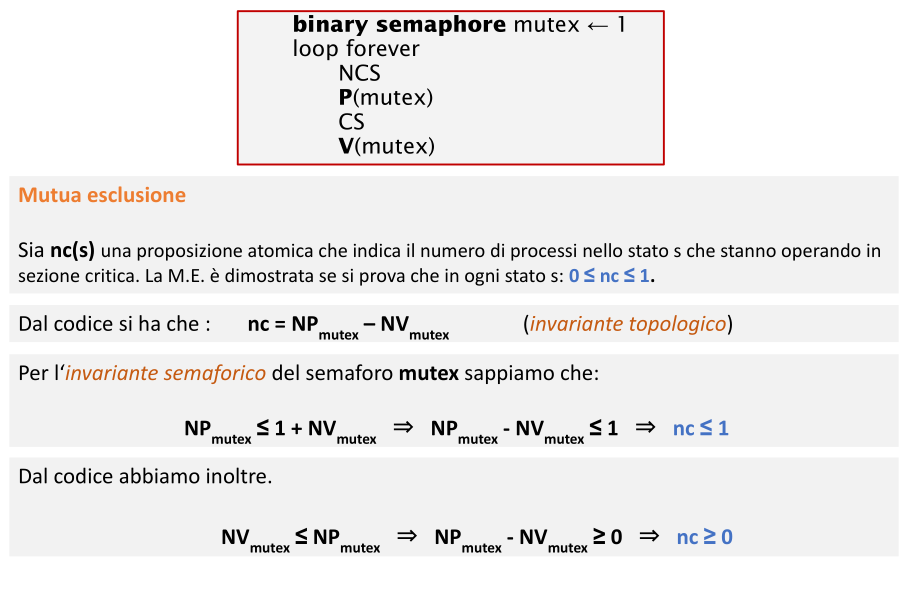
\includegraphics[scale=0.45]{01-IntroduzioneAllaProgrammazioneConcorrente/MEP.png}
\end{center}

Per determinarne la correttezza si costruisce il diagramma degli stati e si sceglie di seguire l'approccio di Ben-Ari:
\begin{itemize}
  \item Mutua esclusione;
  \item Assenza di deadlock;
  \item Assenza di starvation.
\end{itemize}

\begin{center}
    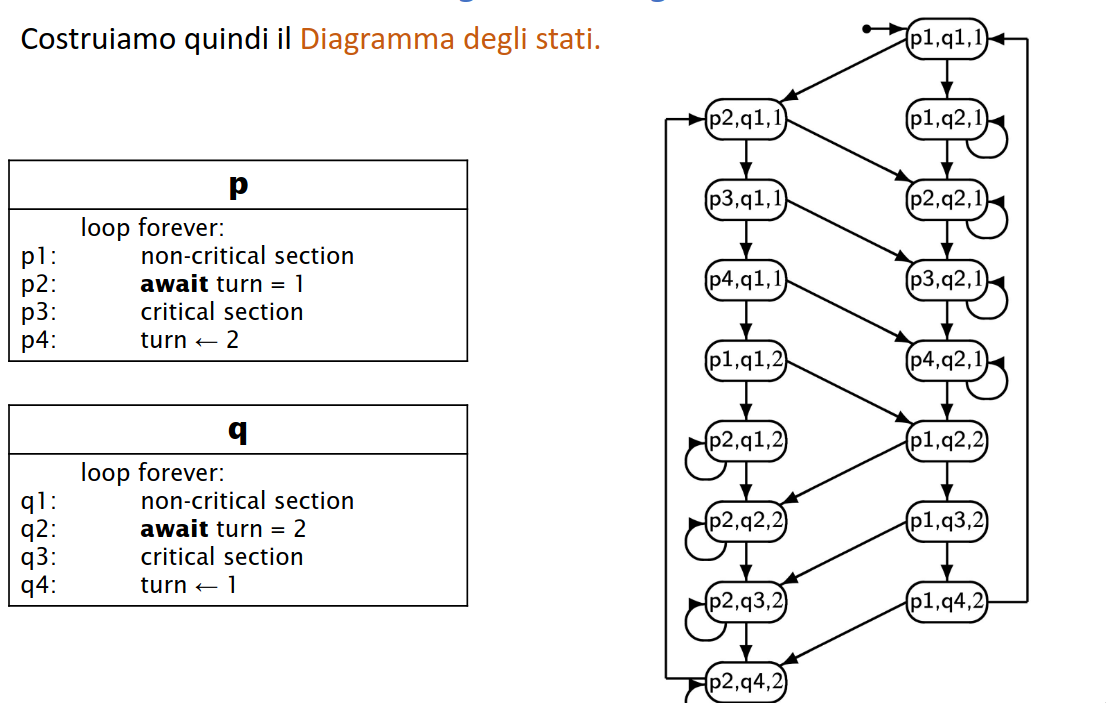
\includegraphics[scale=0.4]{01-IntroduzioneAllaProgrammazioneConcorrente/MEP2.png}
\end{center}

\paragraph{Mutua esclusione:} è sufficente verificare che nel diagramma non esistono stati in cui p e q siano entrambi in sezione critica, ossia stati del tipo (p3, q3, *).


\begin{center}
    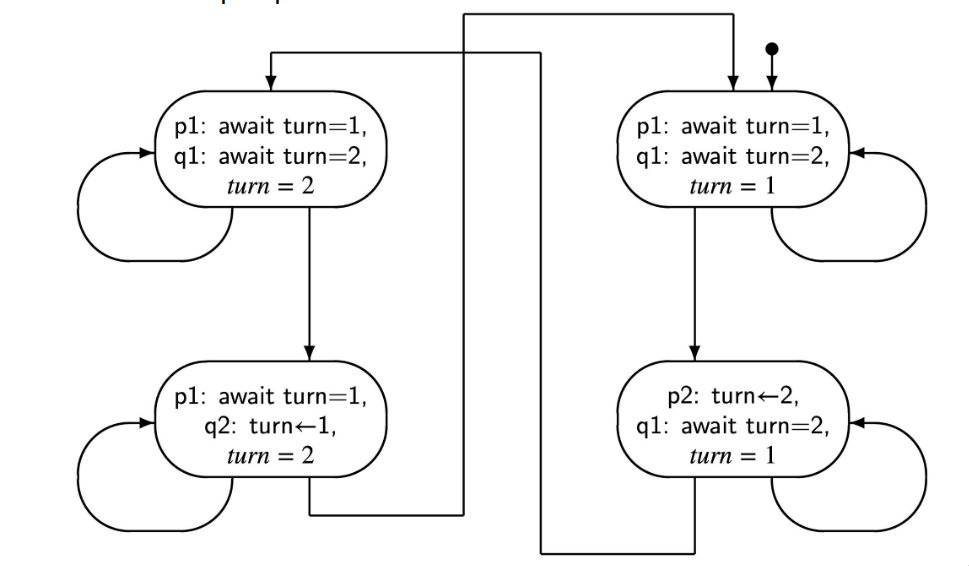
\includegraphics[scale=0.45]{01-IntroduzioneAllaProgrammazioneConcorrente/MEP3.png}
\end{center}

\paragraph{No deadlock:} si utilizza una versione semplificata del diagramma degli stati non considerando la CS. Si vede che ogni stato ha sempre un'uscita.

\paragraph{No starvation:} questo non è vero perché non si ha un progresso garantito al di fuori della CS.

}

\ex{Mutua esclusione}{

Consideriamo un altro algoritmo che non utilizza turn, ma wantp e wantq per indicare se un processo si trova in sezione critica. 

\begin{center}
    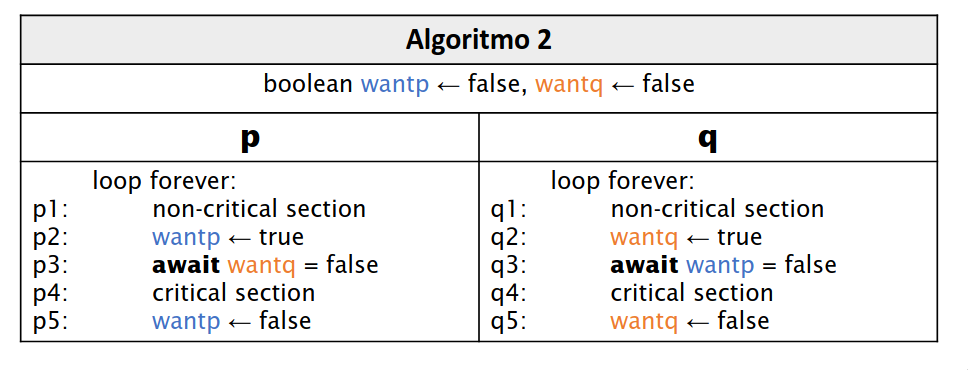
\includegraphics[scale=0.45]{01-IntroduzioneAllaProgrammazioneConcorrente/MEP4.png}
\end{center}

Questo algoritmo garantisce la mutua esclusione però può dare origine a deadlock.


\begin{center}
    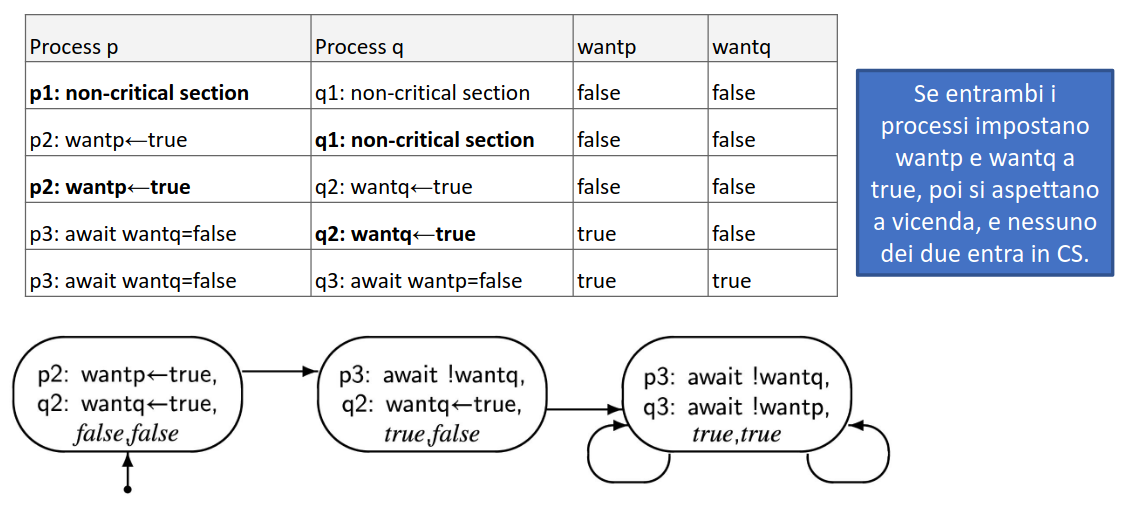
\includegraphics[scale=0.4]{01-IntroduzioneAllaProgrammazioneConcorrente/MEP5.png}
\end{center}


}

\nt{entrambi questi algoritmi sono scorretti. Si deve usare l'algoritmo di Dekker (proposto da Dijkstra nel 1965) che usa sia wantp/wantq che tuen per stabilire quale dei due processi abbia il diritto di insistere nel tentativo di accesso.}

\ex{Algoritmo di Dekker}{
  
\begin{center}
    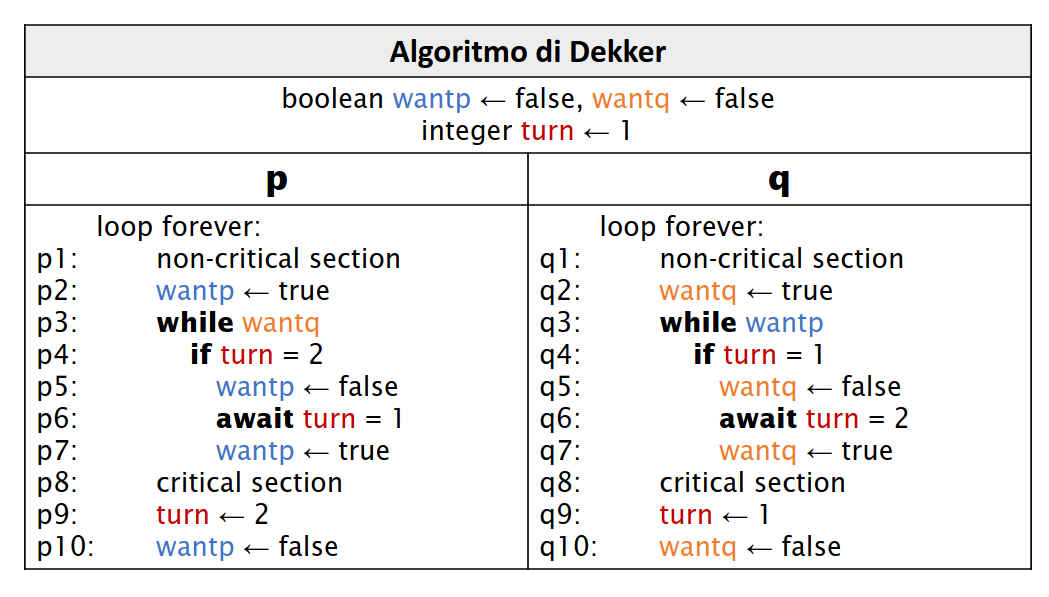
\includegraphics[scale=0.4]{01-IntroduzioneAllaProgrammazioneConcorrente/Dekker.png}
\end{center}

La sua correttezza può essere provata dal diagramma degli stati.

Per provarla in maniera informare si può ragionare per assurdo sulla mutua esclusione: supponiamo che entrambi i processi siano in CS. Uno dei due sarà entrato per primo, supponiamo q (quindi wantq = true). Ora se p entra in CS prima che q ne esca dovrebbe esistere un istante in cui wantq = false mentre q è in CS, ma ciò è assurdo.

Per l'assenza di deadlock si suppone che entrambi i processi vogliano entrare nel ciclo while. Le variabili wantp e wantq sono entrambe true e si suppone turn = 2. Il valore di turn sarà modificato solo quando q uscirà dalla CS. Quindi il processo p dovrà eseguire p5 ed entrare nel ciclo await. Non c'è nulla che ostacoli q a uscire dal while ed entrare in CS.

Per l'assenza di starvation si suppone che il processo p voglia entrare in CS e il processo q sta eseguendo in NCS, p entra. Se invece il processo q esegue in CS o nel prologo/epilogo, per ipotesi prima o poi termina e pone turn = 1 e wantq = false, quindi p può entrare.

}

\nt{Nel 1981 Peterson propose una variante dell'algoritmo di Dekker più semplice e più generale. Ince di usare turn utilizza una variabile last per indicare chi è stato l'ultimo a provare ad accedere: questo determina la priorità di accesso.}

\ex{Algoritmo di Peterson}{
  
\begin{center}
    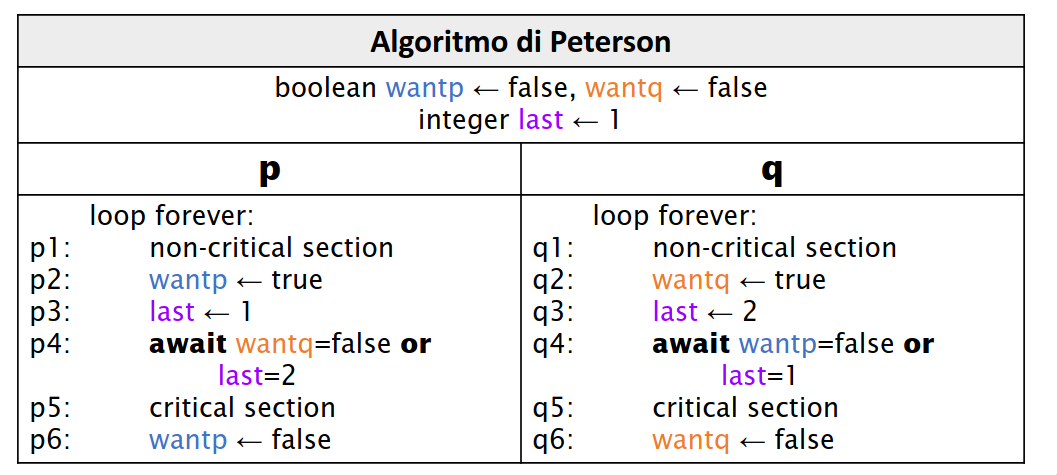
\includegraphics[scale=0.4]{01-IntroduzioneAllaProgrammazioneConcorrente/Peterson.png}
\end{center}

\begin{center}
    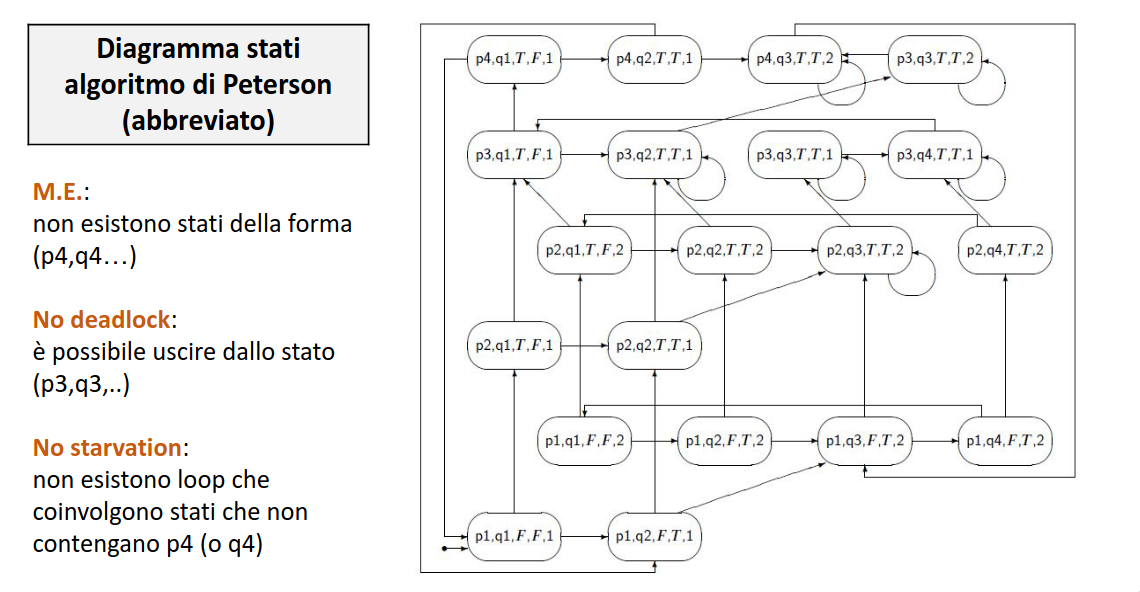
\includegraphics[scale=0.4]{01-IntroduzioneAllaProgrammazioneConcorrente/Peterson2.png}
\end{center}


\begin{center}
    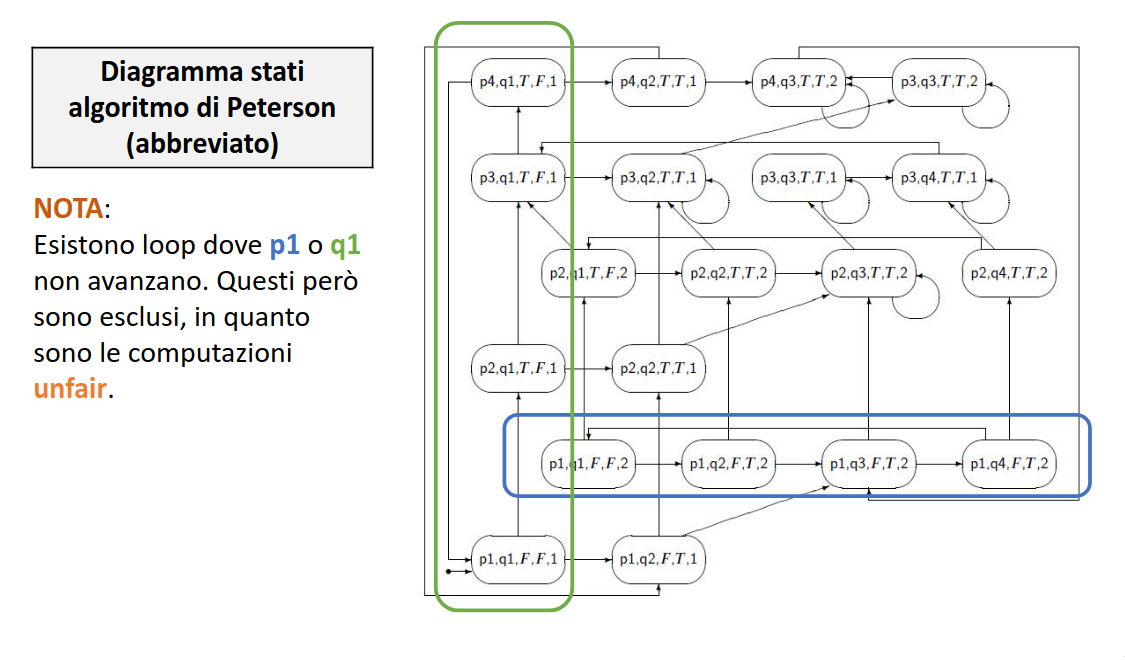
\includegraphics[scale=0.4]{01-IntroduzioneAllaProgrammazioneConcorrente/Peterson3.png}
\end{center}
}

\nt{Nelle moderne CPU multi-core gli algoritmi di Dekker e Peterson non funzionano più (almeno non nella forma vista precedentemente). Perché:
\begin{itemize}
  \item Coerenza della memoria per codice sequenziale per core;
  \item Utilizzo della cache intermedia;
  \item Servono le memory fences (per sincronizzare le cache intermedie).
\end{itemize}
}

\subsection{Statement Atomici Particolari}

Fino a ora abbiamo supposto l'utilizzo di istruzioni atomiche di assegnamento (write e read). Esistono istruzioni atomiche particolari che permettono di realizzare facili ed efficienti meccanismi di sincronizzazione:

\begin{itemize}
  \item test-and-set(common, local);
  \item exchange(a,b);
  \item fetch-and-add(common, local, x).
\end{itemize}

\nt{Questi statement sono tali che durante la loro esecuzione accedono direttamente in memoria centrale (no cache) e non rilasciano il controllo del bus. Così evitano interleaving di operazioni di write e read da parte di altri processi.}
\pagebreak
\ex{test-and-set}{
  
\begin{center}
    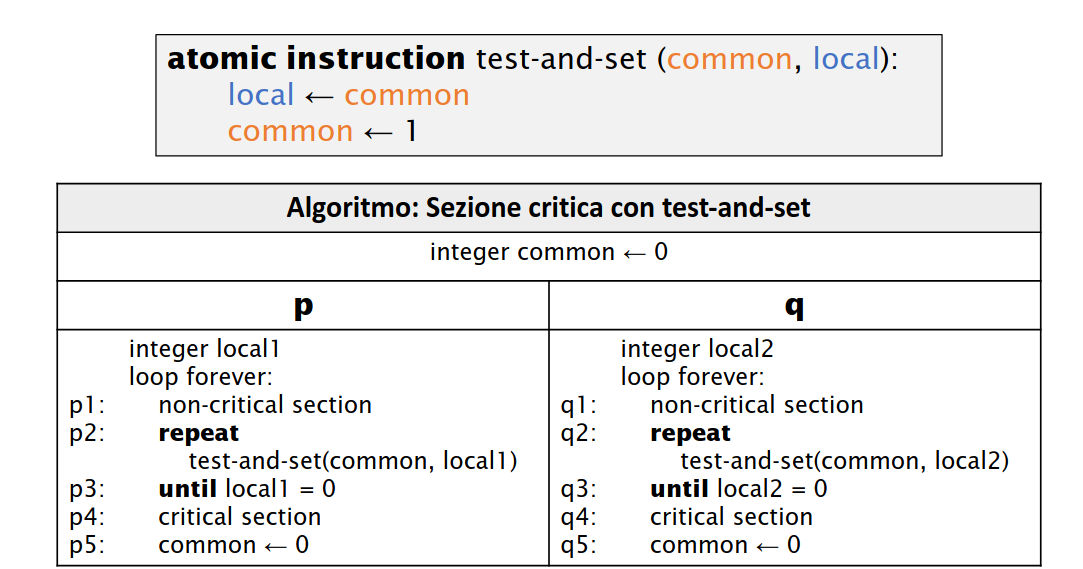
\includegraphics[scale=0.4]{01-IntroduzioneAllaProgrammazioneConcorrente/TS.png}
\end{center}
}

\subsection{Invarianti e Predicati}

Per provare la correttezza di un programma concorrente si può usare l'induzione su \fancyglitter{proprietà invarianti}.

\dfn{Invariante}{
  Un \newfancyglitter{invariante} è una formula A in un qualche sistema formale che ha la proprietà di \newfancyglitter{essere sempre vera in ogni punto di qualsiasi computazione}.
}

\cor{Predicato}{
  Un \fancyglitter{predicato}, chiamato anche \fancyglitter{proposizione atomica}, è un'espressione booleana che può essere valutata avendo a disposizione la tupla delle variabili di stato dei processi, e i loro control pointers.
}

\nt{Le formule A che verranno utilizzate sono anche proposizioni atomiche.}

\clm{Predicati e invarianti}{}{
  Un predicato (proprietà) A è invariante se è vera in ogni punto di qualsiasi computazione.
}

\qs{}{
  Come si dimostra che una proprietà A è un'invariante?
}

\paragraph{Risposta:} la prova che A è un'invariante si fa \fancyglitter{per induzione} sugli stati di tutte le computazioni. Si prova che A vale nello stato iniziale (passo base) e si suppone che A valga in uno stato s e in tutti gli stati precedenti a s (ipotesi induttiva) e si dimostra che vale anche in ciascuno dei possibili stati successivi (passo induttivo).

\nt{In uno programma concorrente gli stati successori possono essere più di uno (per via dell'interleaving) quindi il passo induttivo deve essere verificato per tutti i possibili successori.}

\ex{Invarianti}{

Consideriamo il programma costituito da un unico processo plus; siano:

\begin{itemize}
  \item \textbf{val(x)} il valore della variabile x in uno stato s della computazione;
\item \textbf{val(y)} il valore della variabile y in uno stato s della computazione;
\end{itemize}

Si vuole provare che la formula:

$$0 \leq val(x) - val(y) \leq 1$$
è un \fancyglitter{invariante} del programma.

\begin{center}
    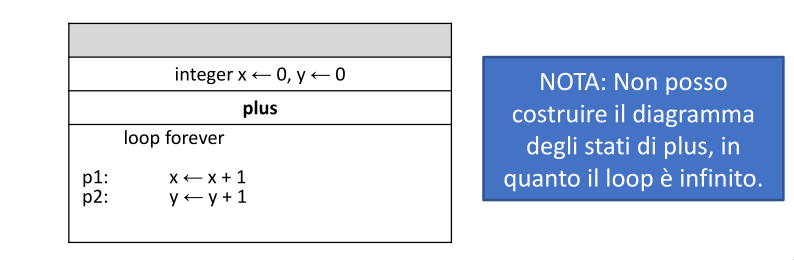
\includegraphics[scale=0.25]{01-IntroduzioneAllaProgrammazioneConcorrente/INV.png}
\end{center}

Si introducono le notazioni:

\begin{itemize}
  \item Npi (i:1..2): variabili intere che in ogni stato indicano il numero N di esecuzioni di pi fino a quel punto completate;
  \item pi (i:1..2): proposizione atomica vera se il control pointer del processo plus vale pi.
\end{itemize}

\begin{center}
    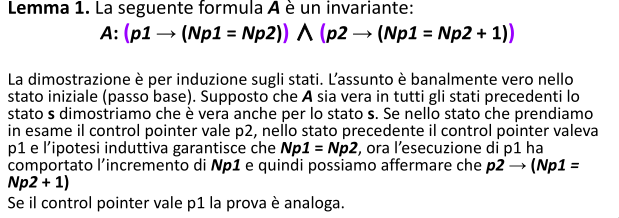
\includegraphics[scale=0.5]{01-IntroduzioneAllaProgrammazioneConcorrente/INV1.png}
\end{center}

Dal Lemma 1 si può dedurre che in ogni stato vale l'Invariante

$$0 \leq Np1 - Np2 \leq 1$$

Un'invariante che si basa sull'ordine delle istruzioni di un processo viene indicato come \fancyglitter{invariante topologico}.


\begin{center}
    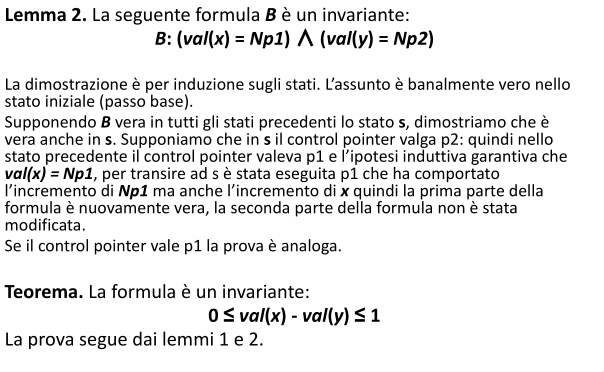
\includegraphics[scale=0.5]{01-IntroduzioneAllaProgrammazioneConcorrente/INV2.png}
\end{center}


}











